%\documentstyle[11pt,epsf]{article}
%\documentclass[preprint]{aastex}
\documentclass[10pt, preprint]{aastex}
\usepackage{epsfig}
\usepackage{epsf}
\usepackage{graphicx}% Include figure files
\usepackage{dcolumn}% Align table columns on decimal point
\usepackage{pbox}

\pagestyle{plain}

\parskip=-1.0pt
\catcode`\@=11 % This allows us to modify PLAIN macros.
\def\Ch{{\it Chandra }}
\newcommand{\beq}{\begin{equation}}
\newcommand{\eeq}{\end{equation}}        
\def\lsim{\mathrel{\mathpalette\@versim<}}
\def\gsim{\mathrel{\mathpalette\@versim>}}
\def\la{\mathrel{\mathpalette\@versim<}}
\def\ga{\mathrel{\mathpalette\@versim>}}
\def\@versim#1#2{\vcenter{\offinterlineskip
        \ialign{$\m@th#1\hfil##\hfil$\crcr#2\crcr\sim\crcr } }}

\def\revtex@ver{4.0}	
\def\revtex@date{25 Apr 95}	
\def\revtex@org{AAS}		
\def\revtex@jnl{AAS}		
\def\revtex@genre{preprint}	
\typeout{\revtex@org\space \revtex@genre\space substyle,
v\revtex@ver\space <\revtex@date>.}
\def\revtex@pageid{\xdef\@thefnmark{\null}
\@footnotetext{This \revtex@genre\space was prepared with the
		   \revtex@org\space \LaTeX\ macros v\revtex@ver.}}
\def\references{{\center \Large REFERENCES}
%\def\references{\section{References}
%\def\references{\subsection*{REFERENCES}
\bgroup\parindent=\z@\parskip=\itemsep
\def\refpar{\par\hangindent=3em\hangafter=1}}
\def\endreferences{\refpar\egroup\revtex@pageid}
\def\thebibliography#1{\subsection*{REFERENCES}
\list{\null}{\leftmargin 3em\labelwidth\z@\labelsep\z@\itemindent -3em
\usecounter{enumi}}
\def\refpar{\relax}
\def\newblock{\hskip .11em plus .33em minus .07em}
\sloppy\clubpenalty4000\widowpenalty4000
\sfcode`\.=1000\relax}
\def\endthebibliography{\endlist\revtex@pageid}
\def\@biblabel#1{\relax}
\def\@cite#1#2{#1\if@tempswa , #2\fi}
\def\reference{\@ifnextchar\bgroup {\@reference}
	{\@latexerr{Missing key on reference command}
	{Each reference command should have a key corresponding to a markcite somewhere in the text}}}
\def\@reference#1{\relax\refpar}

\newcommand{\lya}{Ly$\alpha$\ }
\newcommand{\etal}{et al.\ }

\catcode`\@=12 % at signs are no longer letters

\def\apj{ApJ}                 % Astrophysical Journal
\def\apjl{ApJL}               % Astrophysical Journal, Letters
\def\apjs{ApJS}               % Astrophysical Journal, Supplement
\def\mnras{MNRAS}             % Monthly Notices of the RAS
\def\aap{A\&A}                % Astronomy and Astrophysics
\def\aaps{A\&AS}              % Astronomy and Astrophysics, Supplement 
\def\aj{AJ}                   % Astronomical Journal
\def\physrep{Phys.~Rep.}      % Physics Reports
\def\nat{Nature}              % Nature
\def\araa{ARA\&A}             % Annual Review of Astronomy and Astrophysics
\def\pasj{PASJ}               % Publ.Ast.Soc.Japan
\def\prd{Phys. Rev. D}        % Phys.Rev.D
\def\prl{Phys. Rev. Lett.}    % Phys.Rev.D

\textwidth 6.35 in
\evensidemargin 0.05in
\oddsidemargin 0.05in
%\leftmargin 1.05in
%\rightmargin 1.05in
\topmargin 0.2in
\textheight 8.8in 
\topmargin -.5in


\begin{document}
\input epsf

\title{Cosmology from Non-Linear Weak Lensing}

\author{PI: Zolt\'an Haiman}

\affil{Department of Astronomy, Columbia University}

\section{Summary of objectives} \label{sec:goals}

One of the most pressing problem in modern physics is the nature of
the so-called dark energy, responsible for the accelerated expansion
of the universe.  A promising method to study dark energy is the
measurement of the subtle distortions in the shapes of distant
background galaxies. These distortions are caused by gravitational
lensing, and their statistical properties depend on the physical
nature of dark energy.  Lensing data of unprecedented precision will
be available in the next decade from several large Astronomical
surveys.  The power spectrum of the distortion field (often referred
to as ``cosmic shear'') promises to be among the most powerful future
cosmological probes, and there are indications that higher-order
statistics extract at least a comparable amount of complementary
information from non-Gaussian features.  However, the total
cosmological information content of lensing datasets have not yet been
understood.

Here we propose to use a large suite of cosmological ray-tracing
simulations to create a library of simulated lensing maps, and to
study their cosmological information content.  In particular, our goal
is to clarify how much information is present in these maps beyond
cosmic shear, by examining and combining several different non-linear
statistics.  These simulations form the basis of the NSF proposal
``Cosmology from Non-Linear Weak Lensing'', AST \#1210877, awarded to
the PI for the period 07/01/2012-06/30/2015.  In our on-going work, we
have already created a small suite of simulations, and demonstrated
the utility of several different non-linear statistics.  The
simulation pipeline we have developed has been tested and is now ready
to be deployed, to create the much larger suite of runs required for
our science goals.

In particular, with the simulations proposed here, we will be able to
achieve the following:

\begin{enumerate}

\item The first competitive weak lensing survey has recently been
  completed by the Canada-France-Hawaii Telescope Lensing Survey
  (CFHTLS), and their results have been made public
  \citep{CFHTLS2012}.  While this survey covers only $\approx 150$
  square degrees and includes $\approx$ six million galaxies
  ($\sim1\%$ of the survey planned by LSST; \citealt{LSSTbook}), the
  measured cosmic shear has yielded competitive cosmology constraints
  \citep{Kilbinger2013}.  We will create a simulation suite tailored
  to CFHTLS, and use it to extract cosmological information from the
  non-linear features measured in this survey.

\item With an additional set of simulations, we will increase the
  precision of our measurement of the nonlinear lensing observables,
  and their covariance matrix.  This will allow us to create and
  validate a precision emulator of various WL statistics, analogous to
  an existing emulator for the matter power spectrum \citep{CoyoteII},
  which can be used by other groups in analyzing real WL data in
  larger surveys.  Our simulation library and emulator will be
  necessary to realize the full potential of LSST and other future
  weak lensing datasets and will be released to the public.

\end{enumerate}

The NSF grant mentioned above has supported Columbia University
graduate students Jia Liu (Astronomy Department) and Andrea Petri
(Physics Department), and the simulations proposed here are a
necessary ingredient of their PhD theses.


\section{Scientific motivation: dark energy}

Arguably the greatest puzzle facing modern physics is the physical
nature of dark energy \citep{Tetal03}. This component accounts for
$\sim 70$ percent of the mass--energy density in the universe, and has
caused the expansion of the universe to speed up over the last several
billion years of cosmic history. Despite the fundamental importance of
dark energy (DE), we still know little about its physical nature.  DE
has been conjectured to be associated with phenomena as disparate as
quantum fluctuations of the vacuum, different types of exotic fields
or particles, or a modification of general relativity theory on cosmic
scales.  Our goal in this project is to significantly enhance the
utility of astronomical tools, specifically the statistics of weak
gravitational lensing, in distinguishing between these various
possibilities.  Unlocking the mystery of DE will undoubtedly have
far--reaching implications for fundamental physics.

There are several astronomical approaches to determining the nature of
DE \citep{DETF}.  In general, the presence of DE has an impact on the
expansion rate and the curvature of the universe as a whole.  The
expansion rate and curvature, in turn, can be measured by various
geometric methods, which, in general, require measurements of
distances to distant light sources. DE also affects the growth of local
inhomogeneities -- beginning with the small perturbations in an almost
perfectly smooth initial universe, and leading to the equilibrium
structure of highly non--linear objects, collapsed under their
self--gravity.  Therefore, precise measurements of the inhomogeneities
in the mass--energy distribution provides an alternative method to
study DE.

Learning the nature of DE is one of the highest priorities of the
Astronomy community, with numerous groups around the world devoting
significant resources to the enterprise.  These include experiments
using ground-based and space telescopes whose costs are in the
billion-dollar range.\footnote{Examples include the forthcoming Large
  Synoptic Space Telescope, funded by the NSF and the DOE, and the
  {\it Euclid} satellite being built by the European Space Agency,
  both planned for around the end of this decade.  See, e.g.,
  \citet{Munshireview} for a review of planned instruments and more
  details.} Among the top 4-5 techniques being pursued, weak
gravitational lensing\footnote{Weak gravitational lensing is often
  referred to simply as weak lensing, hereafter abbreviated as WL.}
stands out as especially promising, because of its high statistical
precision, and because it combines sensitivity to both the global
expansion rate/curvature, and to the growth of inhomogeneities.  Our
proposal will explore a possible significant improvement of this
technique, using data that will already be collected (and therefore at
very little or no additional experimental cost).

\section{Weak gravitational lensing: the basic method}

Weak gravitational lensing is the slight distortion in the images of
background galaxies, as the photons they emit travel on the slightly
curved paths predicted by general relativity through the inhomogeneous
mass distribution, before they enter our detectors here on Earth.
This tends to cause a ``shear'': if an intrinsically circular galaxy
is placed behind a massive foreground lump, its image will appear
stretched into an ellipse, as illustrated in Figure 1.  This is
analogous to distortions in an image caused by an optical lens; note,
in particular, that the stretching is in the tangential direction (as
measured from the position of the lens projected on the sky).

%\vspace{0.5\baselineskip}
\begin{figure}[t] \label{fig:a2212} \begin{center}
%\epsfig{file=a2218.ps, angle=0, height=3in}
%\includegraphics[width=8cm]{a2218.pdf}
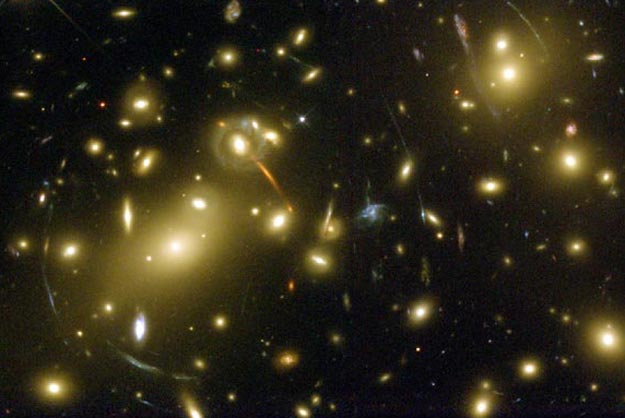
\includegraphics[width=8cm]{a2218c_hst.jpg}
\caption{\it The
  phenomenon of strong gravitational lensing, as seen in an image
  taken with the {\it Hubble Space Telescope}.  The arclets forming a
  circle are the images of background galaxies, distorted by the
  invisible dark matter halo surrounding a massive galaxy cluster in
  the foreground (credits: \citealt{Kneib+1996}).  We propose to use
  the much more subtle weak lensing distortions, detected
  statistically, to probe the nature of dark
  energy.}  \end{center} \vspace{-2\baselineskip}\end{figure}

If we knew the intrinsic shapes of many background galaxies, we could
directly infer, from their observed distortions, the
mass--distribution within the intervening lump of matter.  Of course,
we do not know the intrinsic shape of any individual galaxy.  However,
this does not present a fundamental difficulty: it just means we have
to resort to statistical measurements (the only assumption required is
that galaxies are intrinsically randomly oriented).  In Figure 2, we
illustrate the shear maps that may be expected in two different
cosmological models. These models, in particular, are parameterized by
the equation of state, i.e., the ratio of the pressure and the energy
density, $w\equiv p/\rho$, of the DE. There is a difference between
the two panels, discernible by eye, with the universe with
``stronger'' dark energy (i.e. with more negative pressure, in the
left panel) producing stronger shear.


\begin{figure}[t]
\begin{center}
%\includegraphics[width=8 cm]{fig1a.jpg} \includegraphics[width=8 cm]{fig1b.jpg}\\
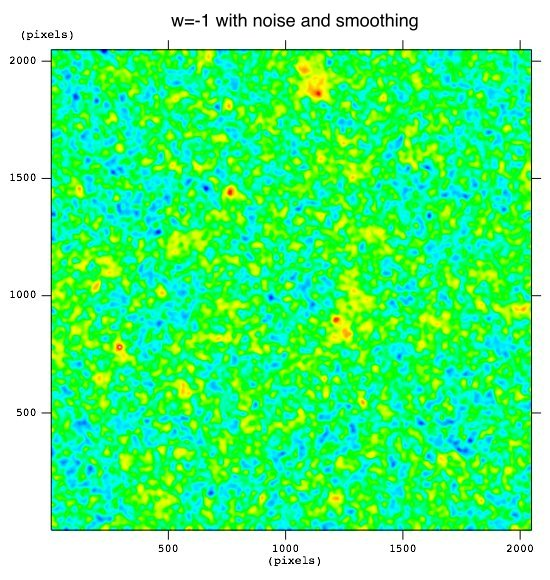
\includegraphics[width=8 cm]{fig1c.jpg} 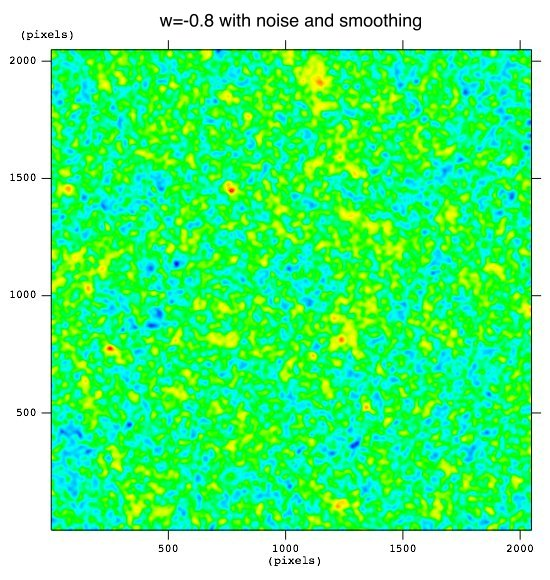
\includegraphics[width=8 cm]{fig1d.jpg}
%\hfill
\vspace{-1.5\baselineskip} \caption{\textit{Examples of shear maps
    from our simulations. We first follow the growth of cosmic
    structures in 3D with an N-body code with $512^3$ particles. We
    then trace the trajectories of light rays, coming from
    hypothetical distant galaxies in each pixel, as they are bent by
    foreground structures.  Each map represents a $3.5\times3.5$
    degree patch of the sky.  Noise has been added due to the random
    intrinsic shapes and orientations of the background galaxies, and
    the maps have been smofothed with a 1-arcminute Gaussian filter.
    The left panel, showing a map for dark energy with more negative
    pressure ($w=-1$), exhibits visibly more structure at high shear
    (in yellow and red) than the right panel (less negative pressure,
    with $w=-0.8$).  Adapted from our existing work \citep{KHM09}. }}
\end{center}
\vspace{-1\baselineskip}
\end{figure}

%\begin{figure}[h]
%\label{fig:viewgeom}
%\begin{center}
%\epsfig{file=fig2a.ps, angle=0, height=3.in}
%\epsfig{file=fig2b.ps, angle=0, height=3.in}
%\caption{\em The weak lensing distortion pattern in two different
%cosmological models.  The short line segments shown in these
%theoretical calculations show the direction and magnitude of the shear
%at each location of the sky, after taking into account the projected
%mass fluctuations in the foreground.  The left panel assumes an
%``Einstein de-Sitter'' universe with the DM having critical
%density. The right panel assumes an open universe, with the DM density
%reduced by a factor of three (credits: B. Jain, et al. 2000,
%Astrophys. J., 530, 547).}
%\end{center}
%\end{figure}

\section{Weak lensing as a probe of dark energy}

There are several astronomical surveys planned to cover large regions
(up to half) of the sky in the future, detecting hundreds of millions
of background galaxies, and measuring their shapes precisely (as
mentioned abvove, the largest existing survey is $\approx$1\% of this
size).  This has motivated theoretical studies to assess how such
giant surveys could be used to probe DE properties.  Such studies
essentially predict statistical properties of the expected WL
distortion pattern, from the inhomogeneities that would be present in
a given cosmological model with a particular amount and form of DE.
One can then go backward and assess how tightly a measured distortion
pattern can constrain the DE models.

For example, because of its negative pressure, the presence of DE
accelerates the overall expansion of the universe, and slows down the
growth of inhomogeneities.  Given the known level of inhomogeneities
in the present-day universe, and going backward in time, DE makes mass
fluctuations larger in the past, which increases the weak--lensing
shear. The shear will also evolve less rapidly with time: the
difference in the level of distortion in the shapes of galaxies
located at two different redshifts (i.e. at different distances from
us) will be smaller.  As a result, the equation of state of DE can be
determined from how the rate of growth of structure changes with
time. This would provide an important clue about the physical identity
of DE. For example, the quantum vacuum has a constant $w=-1$, whereas
models in which DE is a new particle generically predict that $w$
changes with cosmic epoch, and is $w>-1$.

\section{Statistical inferences}

The obvious question at this point is: what statistical property of
the 2D lensing shear field $\gamma(\vec{\theta})$ (such as those shown
in Figure 2) should one measure and use?  Such a statistical analysis
can be divided into two types.  The first type uses the power spectrum
(or equivalent two-point statistics, such as the correlation function
$\langle\gamma(\vec{\theta})\gamma(\vec{\theta}+\Delta\vec{\theta})\rangle_{\vec{\theta}}$).
This is motivated by distortions on large angular scales ($\gsim10$
arcminutes), caused by fluctuations in the foreground mass
distribution on correspondingly large spatial scales ($\gsim30$
light-years).  On these scales, the fluctuations, and hence the
distortion patterns, are small - they are in the linear regime, and
can be interpreted relatively easily, with existing (semi)analytic
tools.  Furthermore, because they are linear, the distortions obey the
statistics of random Gaussian fields.\footnote{This is because the
  density fluctuations generated by quantum fluctuations in the early
  Universe were Gaussian, and this crucial property is preserved in
  the linear regime.} Just as a Gaussian with zero mean is
characterized by a single number (the standard deviation), {\it the 2D
  distortion field in the Gaussian limit can be fully characterized by
  two-point statistics.}  Thus, in the Gaussian limit, there would be
no point in measuring any other statistic.

The vast majority of published work in the field falls into the above
category, {\em despite the fact that the lensing field on small scales
  is manifestly and strongly non-Gaussian.} This is because the
lensing distortions on arcminute-scales are dominated by nonlinear
mass fluctuations: e.g. by foreground galaxies, galaxy clusters, and
the strong filamentary dark matter structures in the so-called
``cosmic web''.


\section{Summary of progress to date and need for new simulations}\label{sec:progress}

Our work to date suggests that the amount of information in the
small-scale, nonlinear regime exceeds that in the Gaussian two-point
functions.  Specifically, by creating mock realizations of the
shear field $\gamma(\vec{\theta})$, we have shown that counting the
number density of local maxima \citep{KHM09,Xiuyuan}, measuring a set
of morphological statistics of thresholded random fields known as
Minkowski functionals \citep{Minkowski}, or higher moments of the
shear field \citep{MF-Andrea}, can yield factors of $\approx2-3$
tighter constraints on dark energy parameters, such as $w$, compared
to using only 2-point statistics.

While these are very important results, they must be regarded
collectively as a simple ``proof of principle'' demonstration.  In
particular, the results are based on a limited suite of lensing maps,
derived from a small set of cosmological N-body simulations.  These
simulations were performed on the IBM Blue Gene/L (36,864 CPUs)
supercomputers at the New York Blue facility at Brookhaven National
Laboratory (BNL), which is part of the New York Center for
Computational Sciences. We ran a series of 70 $N$-body simulations
with $512^3$ cold dark matter (CDM) particles each and a box size of
$240h^{-1}$~Mpc, and used our own ray-tracing pipeline (see below) to
create a total of 21,000 lensing maps, each representing a
$3.5\times3.5$ degree patch of the sky. The crucial limitations of
this suite are the following:

\begin{enumerate}

\vspace{-0.25\baselineskip}
\item {\em Insufficient coverage of parameter space.}  Our existing
  suite includes 7 different cosmological models: a fiducial model
  (using the best fit values from the seven-year results by the {\it
    WMAP} satellite; \citealt{Komatsu2011}), as well as six additional
  models, in which three cosmological parameters are varied. In
  particular, we vary the value of the total matter density
  ($\Omega_m$), the amplitude of the primordial density fluctuations
  ($\sigma_8$), and the DE equation of state parameter ($w$), one at a
  time, in either direction away from the fiducial model
  ($\Delta\Omega_m=\pm0.03$, $\Delta\sigma_8=\pm0.05$ and $\Delta
  w=\pm0.1$).  These seven models, however, are insufficient.  First,
  degeneracies likely exist between $\Omega_m$, $\sigma_8$, $w$, and
  parameters we have not yet varied.  A minimal set would include at
  least three additional parameters: the tilt of the power spectrum of
  density fluctuations ($n_s$), the baryon density ($\Omega_b$;
  \citealt{CoyoteII}), as well as allowing the DE equation of state to
  evolve with time ($dw/dz\neq0$).  Second, in order to describe the
  dependence of any specific statistic on even a single cosmological
  parameter, we have found that interpolations based on our 3 existing
  points are insufficient, with different simple interpolation schemes
  yielding different results.

\vspace{-0.5\baselineskip}
\item {\em Insufficient redshift coverage.}  Our current suite
  includes simulated lensing maps only at 3 different redshifts in
  each cosmology ($z_s=1, 1.5$ and $2$).  Real surveys, of course,
  include galaxies with a continuous distribution in distance,
  covering the redshift range ($0<z\lsim2$).  We need to produce mock
  lensing maps over this entire redshift range, with a spacing $\Delta
  z_s\approx 0.04$ comparable to the (photometric) redshift accuracy
  of real surveys - this requires 60 distinct $z_s$ values.

\vspace{-0.5\baselineskip}
\item {\em Insufficient number of lensing maps.}  Our current suite
  includes 1,000 maps at each redshift for each cosmological model.
  We have demonstrated that this results in an important
  limitation. In particular, 1,000 realizations only allow us to
  estimate the covariance matrix of only O(100) observables.  Taking
  the number density of peaks on the 2D lensing maps as an example:
  our work suggests that one can tighten the cosmological constraints
  by combining several different redshifts, smoothing scales, and peak
  heights. Thus, in practice, we will need the covariance matrix for
  more than 100 observables.

\vspace{-0.5\baselineskip}
\item {\em Insufficient number of N-body simulations.}  Finally, as
  mentioned above, our current suite of lensing maps is based on 70
  independent N-body simulations. As a result, we have had to resort
  to the common practice of reusing the same snapshot of a 3D
  simulation box, from the same simulation, several times.  More
  specifically, the cosmic structure represented in a single 3D
  simulation output (at a fixed cosmic time) is randomly shifted and
  rotated, before a 2D projection is created for ray-tracing (see
  below).  While this approach is adopted in virtually all existing
  studies, one still inevitably projects through the same cosmic
  structures multiple times.  Our existing work suggests that the
  resulting maps are not sufficiently statistically independent.

\end{enumerate}

\vspace{-0.25\baselineskip} We propose a new suite of simulations,
with which we can address all of the above issues, all fundamentally
important for an eventual use of non-linear WL statistics.  The Blue
Gene/L at BNL has been decommissioned, and we propose to shift our
production runs to XSEDE Stampede.\footnote{We have benchmarked our
  pipeline on the new Blue Gene/Q facility at BNL and found it to be
  far inadequate for our production runs, due to poor communication
  and I/O with the new disk system, which makes its overall
  performance more than 10 times slower than Stampede. The new
  facility also lacks adequate storage for our purposes.}

\section{Computational methods}
\label{Computational}

Our pipeline to produce mock lensing maps consists of three distinct
steps.  First, we run N-body simulations, to follow the growth of
cosmic structures, producing outputs at several cosmic times.  Second,
at each output, we project the 3D structures onto 2D ``lens planes'',
and solve Poisson's equation in 2D to compute the lensing potential on
these planes.  Third, beginning from the observer, we ``shoot'' light
rays towards fixed angular directions, computing the deflection of the
rays when they cross each lens plane.  For the first of these steps,
we use the public N-body code Gadget-2 \cite{VS05}, whereas for the
second and third steps, we use our own code, written by collaborator
Jan Kratochvil, implementing the algorithm outlined in \citet{H&M01}.
We have benchmarked each of these steps on the XSEDE cluster Stampede,
as explained below and in the ``Code Perfomance and Scaling''
document.

\subsection{N-body Simulations}

Our $N$-body simulations are run with $512^3$ particles each, and a
box size of $240h^{-1}$~Mpc. We have made minor modifications to the
public N-body code Gadget-2 to allow a dark energy equation of state
parameter $w\neq -1$, which can also vary with time ($dw/dz\neq0$) as
well as to compute weak lensing related quantities, such as comoving
distances to the observer.  Gadget's adjustable parameters were
fine-tuned for maximum throughput. Volker Springel, the author of
Gadget, kindly provided us with the initial conditions (IC) generator
N-GenIC. The total linear matter power spectrum, which is an input for
the IC generator, was created with the Einstein-Boltzmann code CAMB
\citep{CAMB} for $z=0$, and scaled to the starting redshift of our
simulations at $z=100$ following the linear growth factor.  The
large-scale structure from the N-body simulations is output as
particle positions in boxes at different redshifts, spaced $80h^{-1}$
comoving Mpc apart, starting at redshift $z=2$; this results in 58
snapshots.

\subsection{Lensing Maps}

The weak lensing maps are created with a standard ray-tracing
algorithm \citep{H&M01}. The particles from each N-body snapshot are
projected onto planes perpendicular to the central line of sight of
the map.  We use the triangular-shaped cloud scheme
\citep{Hockney-Eastwood} to place the particles on a grid on these 2D
density planes; the particle surface density is then converted into
the gravitational potential via the Poisson equation. The algorithm
then follows light rays from the observer back in cosmic time. The
deflection angle, as well as the weak lensing convergence and shear is
calculated at each plane, for each light ray. These depend on the
first and second derivatives of the potential, respectively. Between
the planes, the light rays travel in straight lines.  The maps are
created for $2048\times2048$ light rays, with the lens planes spaced
$80h^{-1}$Mpc apart along the line of sight. The lens planes record
the gravitational potential on a finer $4096\times4096$ grid, to avoid
losing power on small angular scales, as pointed out by
\citet{Sato09}. We have found a similar fall-off, and therefore
increased the resolution on the density planes since our first
publication \citep{KHM09}.  We create pseudo-independent $\approx
3.5\times3.5$ square-degree convergence and shear maps for each
cosmology, by mixing simulations with different random ICs, and by
randomly rotating and shifting the simulation data cubes.

\subsection{Noise, smoothing, and mass reconstruction}

%JL real (not analytical) noise is added.
After the raw maps with the lensing signal are generated, we add
ellipticity noise from the intrinsic shape and random orientations of 
the source galaxies to the maps. We use realistic ellipticity from the 
survey, by randomly rotate the galaxies on the spot.
% pixel by pixel.  We assume the noise is represented by a
%Gaussian random field (with a top-hat filter of pixel size), whose
%amplitude is specific to the number density of galaxies in any
%specific survey. 
Once noise in each pixel is added, we smooth the maps
with a finite version of a 2D Gaussian filter, on smoothing scales
ranging from $\theta_G = 1-10$ arcmin.
%JL add mass reconstruction below.
To prepare for our analysis, we reconstruct the mass maps for 
both simulated maps and CFHTLS maps using the Kaiser Squires 
method\cite{Kaiser1993}.

\subsection{Analysis}

Once the %JL - convergence and shear
mass maps are created, they are ready for
analysis. Our final goal is to compare nonlinear statistics measured
on these maps from various cosmologies with each other and with the
values measured in the CFHTLS survey.  Following our earlier work, the
statistics will include peak counts, moments, and Minkowski
functionals. These are straigthforward to measure on the maps; we
expect to be able to perform these measurements, and analyze the
results either on Stampede, or using local computational resources
(see below).

\vspace{\baselineskip}

In the computational workflow described above, the bottleneck is
generating the N-body simulations.  Each N-body run requires $\approx
780$ SU (benchmarked on Stampede).  By comparison, generating each
lensing map requires $\approx 0.18$ SU.  Since we expect to be able to
create at most 200 sufficiently independent maps per single N-body
run, the total cost of ray-tracing will be $\lsim 36$ SUs per N-body
simulation.  \textit{We therefore emphasize that $\approx 95\%$ of our
  request for computational time is consumed by the N-body runs
  performed with Gadget-2.} This code is being widely used for this
purpose, and is known to scale well.
%In the computational workflow described above, generating the N-body
%simulations consume comparable computing time.
%Each N-body run requires $\approx 780$ SU (benchmarked on Stampede).
%By comparison, generating each single lensing map requires $\approx
%0.18$ SU (see ``Code Performance and Scaling'' document). Since we
%expect to create 4,000 independent maps per single N-body run, the
%total cost of ray-tracing will be $\lsim 720$ SUs per N-body
%simulation.

\section{Justification of Requested Resources}\label{Justification}

\subsection{Deriving Cosmological Constraints from the CFHTLS Survey}.

\begin{figure}[t!]
\label{fig:cfht}
\begin{center}
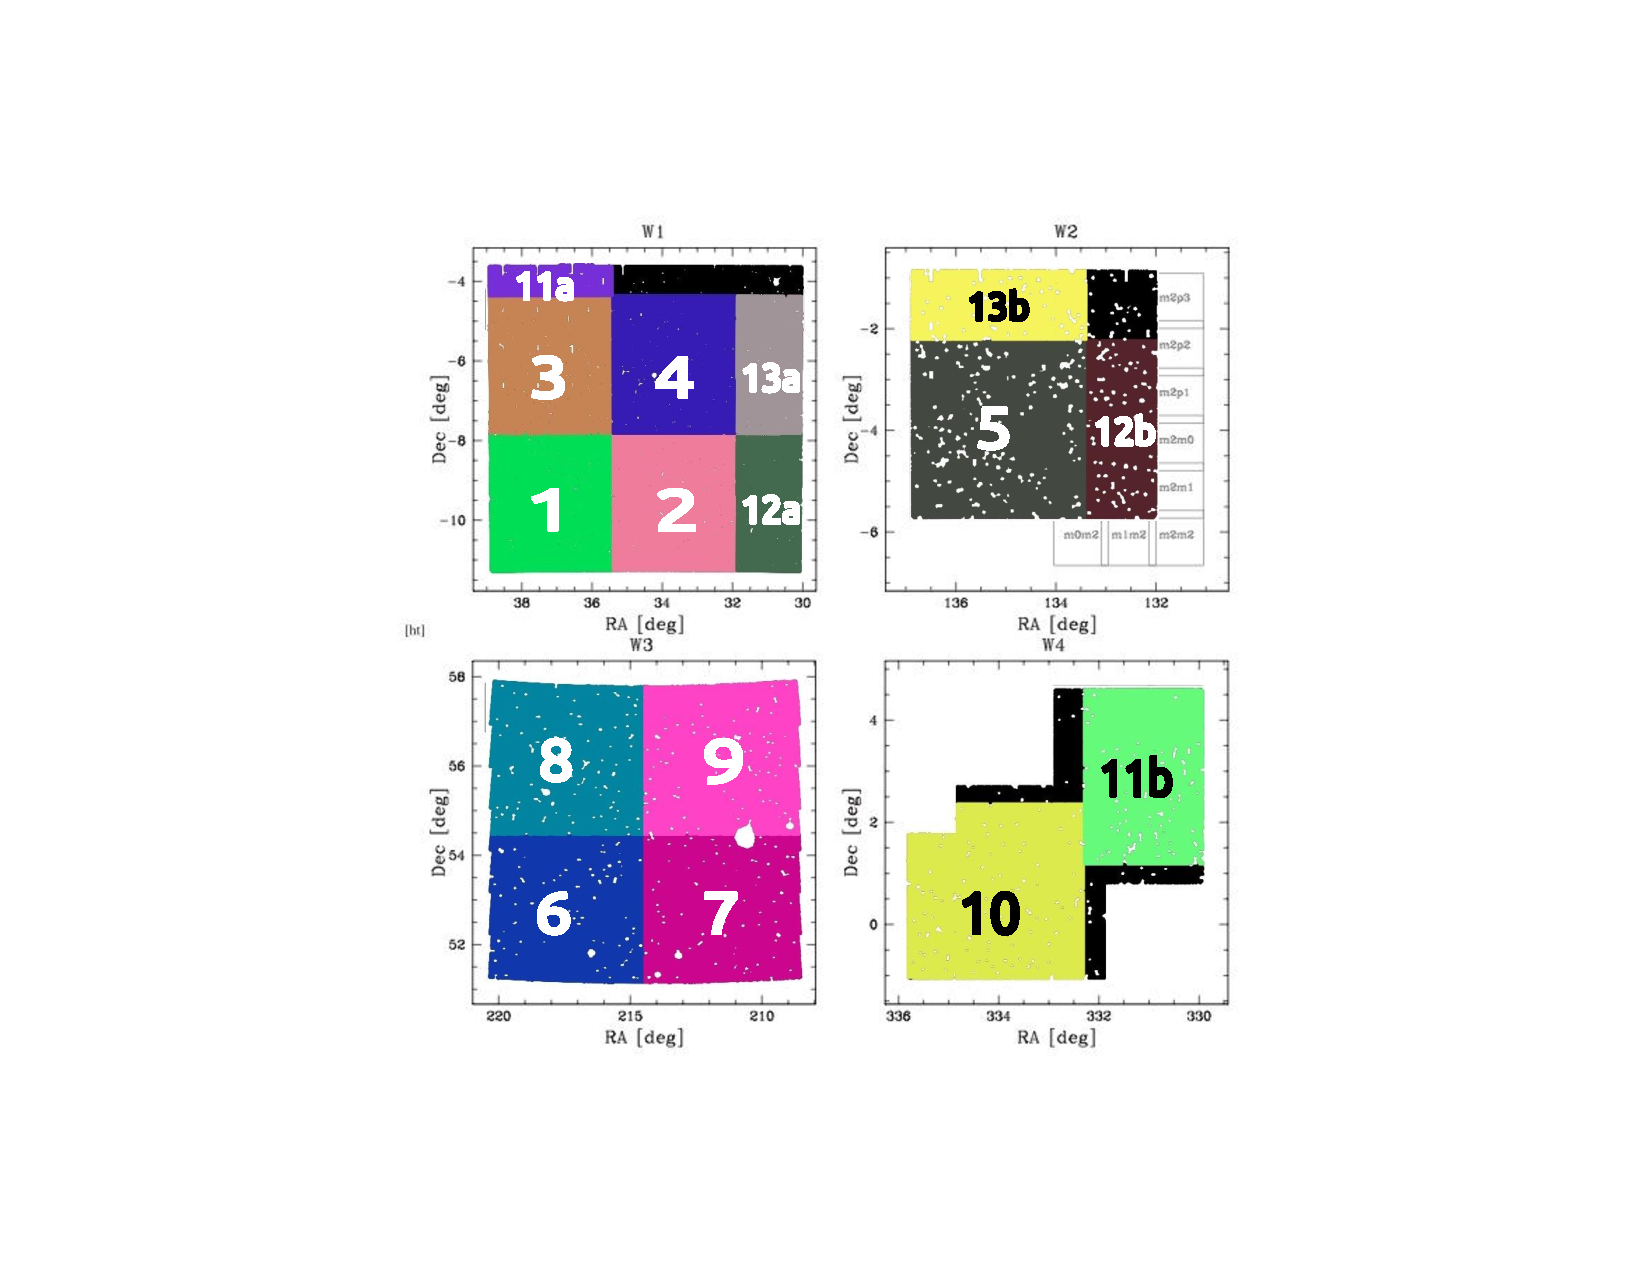
\includegraphics[height=10cm, width=10cm]{CFHTjia.pdf}
\vspace{-4\baselineskip}\caption{\it The four different subfields of
  the CFHTLS survey can be covered by 13 of simulated 3.5$\times$3.5
  degree lensing maps, with some of our maps suitably cut up into
  smaller pieces, as indicated in this figure.}
\end{center}
\end{figure}

As stated in \S~\ref{sec:goals} above, our first goal is to derive
cosmological constratins from nonlinear WL statistics applied to the
CFHTLS survey.  The size of this survey is $\approx 150$ square
degrees, consisting of four distinct regions of the sky.  The survey
area can be explicitly tiled by using 13 of our simulated 12
sq. degree fields, subdividing the CFHT sky coverage into suitable
regions (see Figure~3).  The angular positions and redshifts of the
CFHTLS galaxies are known; we expect to use the 4.2 million galaxies
with accurate photometric redshifts and shape measurements, in the
redshift range $0.2 < z < 1.3$ \citep{Kilbinger2013}.  This number
coincides with the number of pixels in one of our $2,048\times2,048$
pixel maps. Thus the raytracing in the known sky positions of the
CFHTLS galaxies requires a computing time comparable to raytracing to
every pixel in one of our $3.5\times 3.5$ square degree maps.

As described in \S~\ref{sec:progress} above, we wish to include a
total of six cosmological parameters in this analysis.  Sampling a
multidimensional parameter space on a regular grid becomes
computationally forbidding. A more sophisticated distribution of our
simulations in the 6D parameter space is necessary, which samples more
individual parameter values without increasing the number of sampling
points. As a consequence, this results in an irregular grid in the
parameter space. One of these methods is the orthogonal array-based
Latin hypercube sampling, adopted by \cite{CoyoteII} for a similar
application in cosmology.  The interpolation on an irregular grid must
then be done carefully with techniques which are as little biased as
possible by the irregular distribution of the measurement
points. Following the application to the 3D matter power spectrum by
\cite{CoyoteII}, we will employ Gaussian processes for this
interpolation task. We are currently in the process of implementing
this technique.  However, we note that \cite{CoyoteII} haved use 38
simulations to span a five dimensional cosmological parameter
space. In order to accommodate our additional parameter, and to cover
the somewhat larger parameter ranges than adopted in \cite{CoyoteII}
(likely necessary for less accurate present-day survey, such as
CFHTLS), we propose to perform N-body simulations at $N_{\rm
  cosmo}=100$ points in the parameter space.

As also described \S~\ref{sec:progress}, another limitation arises
from the lack of independence between maps, when too few underlying
simulations are used.  In our existing work, we mixed the lens planes
drawn from 5 independent N-body runs in each cosmology. Here we
propose to quadruple this number, and use $N_{\rm sim}=20$ Gadget runs
per cosmology.

Finally, we had a large set of WL maps for our past simulation suite,
consisting of 1,000 12-square-degree fields, yet, as described in
\S~\ref{sec:progress} it has proven not to be enough to overcome the
noise in the covariance matrix. As a result, we were not able to
verify that we extracted all the information present in any given
statistic. In addition to noise suppression techniques in the
covariance matrix, which in the field of weak lensing are only
beginning to be explored, the most obvious solution is to create more
WL maps. Based on our results, we estimate that we need to increase
the number of maps by a factor of 4, and to create 4,000 realizations
of each full CFHT map. As argued above, the entire CFHT area is
roughly equivalent (in terms of the number of independent raytracings)
to a single map we had previously used.  This allows us to recycle
each of our map $\sim 13$ times, resulting in the requirement of
$N_{\rm map}=4,000$ individual 12-square-degree maps per cosmology.

As mentioned above (and shown in the ``Code Performance and Scaling''
document) a single N-body run requires 780 SUs, so that a total of
$N_{\rm cosmo}\times N_{\rm sim}=2,000$ simulations will require 1.56
million SUs.  Creating $N_{\rm cosmo}\times N_{\rm map}=400,000$ maps
will require 72,000 SUs.  The overall requirement of the CFHTLS
analysis will therefore amount to 1.7 million SUs.  We request
long-term storage for all lens planes (69.2TB) and the full 3D
snapshots in a representative run in each of the 100 cosmologies
(25TB).  Each realization for every subfield requires 30MB, so that
12TB will be required for temporary storage of our lensing maps.  The
lensing maps will be downloaded to our local resources for further
analysis.

\subsection{A Nonlinear Weak Lensing Emulator}

Our second goal, stated in \S~\ref{sec:goals} above, is to derive an
emulator, which predicts WL observables sufficiently accurately to be
useful in larger survey, as well as to predict the covariance matrix
of the WL observables to high accuracy, required in obtaining
likelihood functions for future, larger datasets.  

For the measurement of the covariance matrix, we propose to perform an
additional $N_{\rm sim}=500$ simulations of our fiducial cosmological
model.  Based on the results of \cite{Sato09}, who have performed 400
comparable runs to study the non-Gaussian tails in the covariance of
the WL power spectrum, we expect that 1,000 independent simulations
will be required to characterize the covariances of the non-linear
statistics, including the rare non-Gaussian tails, which we expect to
be more significant than for the power spectrum.  This will require
0.78 million SUs.

For accurate measurements of the nonlinear WL statistics in different
cosmologies, we propose to increase the number of maps produced in
each cosmology, by a factor of 10.  As explained above, the computing
time required to produce these additional maps is relatively modest
(0.72 million SU).  However, storage requirements for such a large set
of maps becomes significant (120TB for 4 million maps).  For the
purposes of creating the emulator, we will therefore store only the
derived products on each map (the number of peaks, moments, and
Minkowski functionals measured on each map), which will require $<3$TB.


\subsection{Summary of Computing Time and Disk Space Request}

\begin{table}[t!] \label{tab:summary}
\begin{center}
\begin{tabular}{|c|c|c|c|c|}
\hline
\textbf{Project} & \textbf{Time Required} & \textbf{Storage Space Required}\\ \hline \hline\hline
CFHT: N-body Simulations (2000 runs) & 1.56 million SUs & 25TB (3D data for 100 simulations) \\ \hline 
CFHT: Ray-tracing (400,000 maps)  & 72,000 SUs & 70 TB (lens planes) + 12 TB (maps)\\ \hline
Emulator: N-body Simulations (1000 runs) & 0.78 million SUs & 25TB (3D data for 100 simulations) \\ \hline 
Emulator: Ray-tracing (4 million maps)  & 720,000 SUs & 3 TB (derived products only)\\ \hline\hline\hline
Total & 3,232,000 SUs & 135TB \\ \hline
\end{tabular}
\end{center}
\caption{\textit{Summary of requested computing time and disk storage.}}
\end{table}

In summary, we are asking for 3.5 million SUs, the bulk of which (3.2
million SUs) will be consumed by our N-body simulations, the rest
being required for raytracing, initial condition generation, and map
analysis (we have rounded up the estimate of our figure in
Table~\ref{tab:summary} by $\approx 200,000$SUs to allow for the
latter).  Our storage requirements are 135 TB.  50 TB of these
consists of long-term storage of the full 3D simulation data in 200
N-body runs, and 82 TB for storage of all of the lens planes required
for the CFHT analysis, as well as 400,000 simulated lensing maps.

\section{Local Computing Environment}\label{Local Computing}

We have access to a new High Performance Computing cluster ``Yeti''
shared by the Departments of Astronomy, Statistics, Economics, and
other departments at Columbia University.  This cluster has a total of
1616 cores, shared by 101 nodes (16 cores per node), with memory
ranging from 64-256 GB.  There is an effective storage space of 100
TB.  While this shared resource is insufficient for our production
runs, we expect we will be able to perform our analysis locally on
this machine.

\section{Project Team Qualifications}

PI {\bf Zoltan Haiman} is a Professor of Astronomy at Columbia
University.  He is a theoretical astrophysicist, whose work has
focused on structure formation in the early universe, and in using
galaxy clusters to probe the nature of dark energy and dark matter.
The modifications to Gadget and the raytracing pipeline was written by
collaborator {\bf Jan Kratochvil}, who is currently a postdoctoral
researcher at the University of KwaZulu-Natal in Durban, South Africa.
Over the past year, Kratochvil and Haiman have worked closely with two
Columbia graduate students.  {\bf Jia Liu} is a third-year student in
the Astronomy department, and has focused on issues related to
comparing simulations to observational data. She has already
familiarized herself with the CFHTLS data.  {\bf Andrea Petri} is a
third-year student in the Physics department, and has worked closely
on the simulation pipeline with Kratochvil, including the benchmarking
we have already done on Stampede.



\bibliographystyle{jponew}
\bibliography{refs}

\end{document}






\section{Machine learning}

We will answer the above questions by creating a library of
weak--lensing distortion maps for a suite of DE models.  Briefly, the
procedures are as follows: perform N-body numerical simulations of the
growth of structure in a given model; compute how light from
background galaxies travels and gets deflected in such a universe;
calculate the resulting distortion of images of galaxies; repeat for a
variety of DE models, as expected in different physical theories.  We
will then be able to intercompare these maps, which cover scales from
the linear all the way to the fully nonlinear regime, using different
comparison techniques, statistics and algorithms.

Our approach will be based on ``machine learning''. Our problem is
quite general, in that we are presented with two images, which can
differ either due to random variations (two different realizations of
the WL maps drawn from the same underlying distribution, i.e. in the
same DE model), or due to genuine differences in the underlying DE
model.  The chief difficulty is that we do not know a-priori the best
distinguishing patterns to look for.  Our proposed novel strategy is
to create a large catalog of images (lensing maps) which are multiple
realizations of many different DE models, and feed these images to a
machine learning algorithm.  Such algorithms can be trained to
distinguish between different models based on these trial images.
Once an algorithm has been trained, we can then go back to examine
what distinguishing features have been used, whether they correspond
to the traditional two-point correlation function, or the counting of
peaks, or to something completely unexpected.

\section{Conclusions}

The project is somewhat risky in that there is no guarantee that the
constraints DE can indeed be significantly improved from a machine
learning analysis of the fully nonlinear weak lensing maps. On the
other hand, as discussed above, there are good reasons to believe that
current methods do not capture most of the available information.
Should we find large improvements, this would have a large immediate
impact on experimental cosmology: the specifications of forthcoming
surveys should then be altered in light of the possible new
information.







\begin{figure}[ht]
\label{fig:telescopic}
\begin{center}
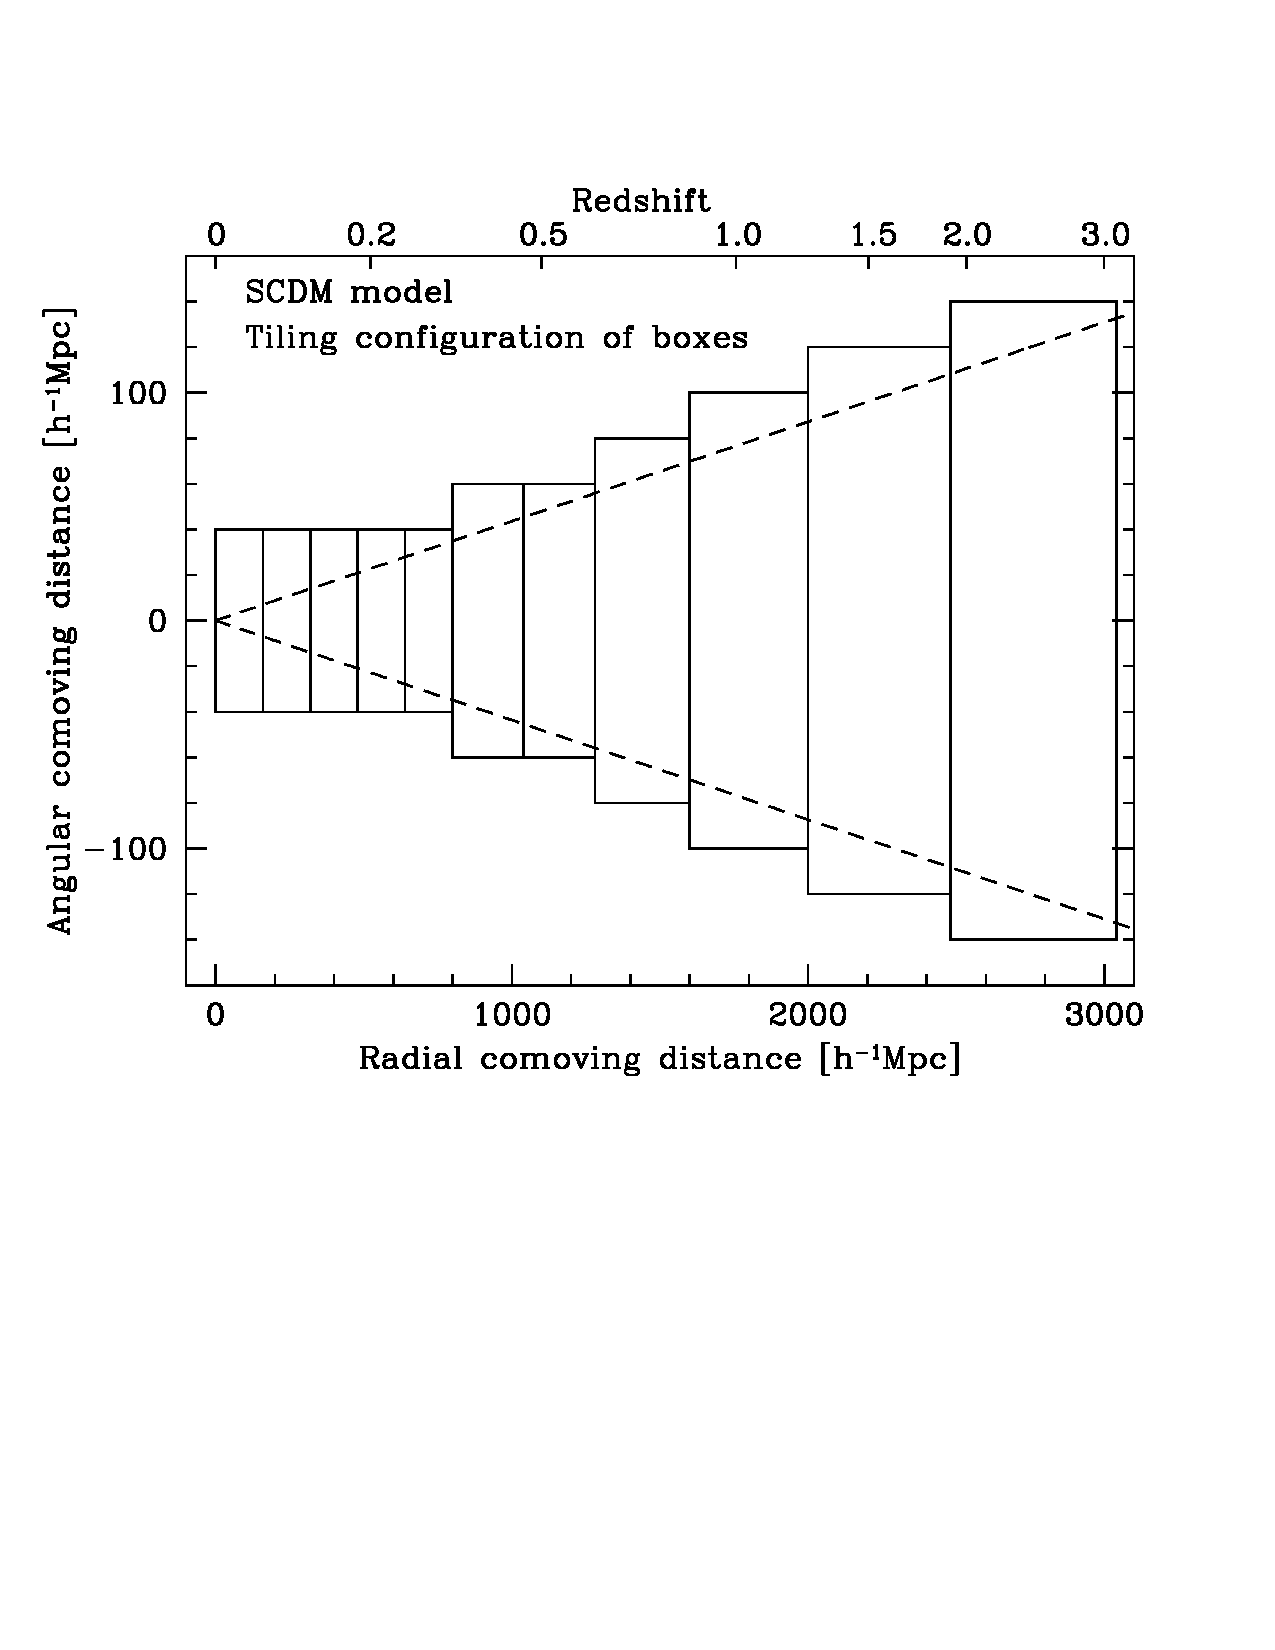
\includegraphics[height=8cm, width=8cm]{HM_0101333_f1.pdf}
\caption{\it Telescopic arrangement of snapshot boxes (particle
position outputs) from N-body simulations are lined up along the line
of sight away from the observer on the left. Boxes from different
simulations with different comoving size of the simulated box, but
same number of particles, are used to efficiently fill out the view
cone (dashed lines). Without such size adjustments, the closest boxes
would be at very poor resolution because of the small opening of the
cone there (figure from \citealt{H&M01}).}
\end{center}
\end{figure}
